% -----
% ARQUIVO: capitulo-03.tex
% VERSÃO: 1.1
% DATA: Janeiro de 2016
%
% CAPÍTULO DE CONCEITOS BÁSICOS DA PROPOSTA
%
% NÃO MEXA NAS SEÇÕES, SOMENTE EDITE O CONTEÚDO.
% -----

\chapter{Conceitos B\'{a}sicos e Estado da Arte}
% #TXT_CONCEITOS
\textbf{Explicando Malware\\
Explicando técnicas de análise de malware: Estática, Dinâmica, Híbrida\\
Explicando técnicas de evasão(?)\\
Explicando Deep Learning\\\\
Entrar no estado da arte para deep learning e análise de malware separadamente ou no caso aqui o estado da arte é Análise de malware com deep learning?}


% Para usar figuras, use sempre o mesmo template abaixo. altere somente:
% 1. os parâmetros do comando \includegraphics[width=•]{•} / tamanho e arquivo
% 2. \caption{*} / para colocar o rótulo da figura em *
% 3. \label{*} / para colocar a chamada para a figura no texto em *
%    TODA figura deve ter uma chamada no texto e esta deve ser feita sempre no formato:
%    Figura \ref{•} (p. ex. "Figura \ref{fig:artigo1}")

\begin{figure}[!h]
	\centering
	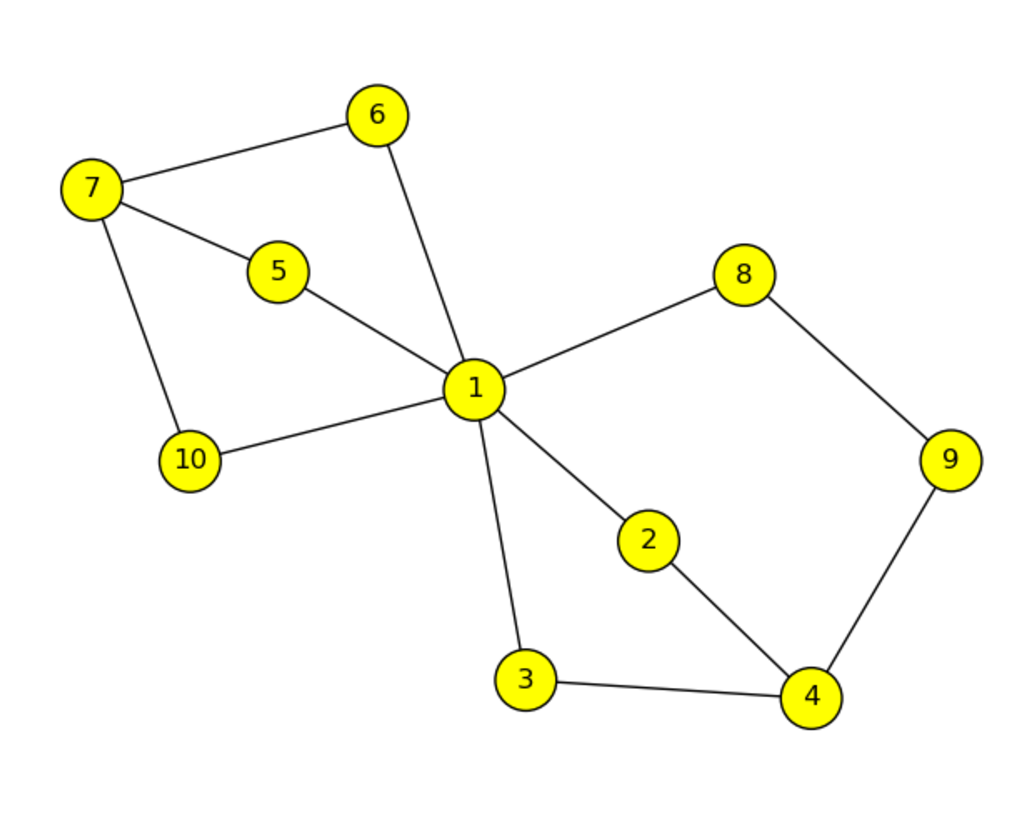
\includegraphics[width=0.4\textwidth]{artigo1.eps}
	\caption{R\'{o}tulo da Figura 1, descrevendo a figura.}
	\label{fig:artigo1}
\end{figure}

\section{Trabalhos Relacionados}
% #TXT_TRABREL
\textbf{Definir paragrafo inicial:} Explicar os problemas da análise de malware: Descrever sobre o gargalo gerado por necessitarmos de um analista especialista para realizar a análise de um arquivo, criando uma demora na atualização dos sistemas de segurança.  Informar que a velocidade que os malwares são criados e alterados, utilizando-se de diversas técnicas de evasão, criam a necessidade de ferramentas automatizadas mais inteligentes e adaptáveis não só aos malwares conhecidos mas também a novos malwares. Mostrar a necessidade da pesquisa na área é cada vez mais importante, visto que agora o potêncial dos danos é ainda maior, já que temos cada vez mais dispositivos com boa capacidade de processamento e acesso a redes rápidas, como smartphones e outros dispositivos (internet das coisas, por exemplo).
Explicar um pouco como o deep learning poderia ajudar na tarefa de extração de característica e criação da hierarquia de representações a partir de dados brutos sem a necessidade de um especialista. Detalhar os trabalhos relacionados (somente deep learning)

Diversos estudos vem sendo conduzidos tanto em inteligência artificial, no desenvolvimento de algoritmos de treinamento e novas arquiteturas de redes neurais com o objetivo de aprender essas hierarquias de representações, tanto em análise de malware, preocupando-se em criar sistemas mais robustos e resistentes às técnicas de evasão empregadas por códigos maliciosos. Também podemos observar vários trabalhos que se utilizaram de técnicas de Deep Learning aplicadas ao problema da análise de malware, seja por análise estática, dinâmica ou híbrida. Abaixo, comentamos um pouco sobre esses trabalhos. 

\subsection{Trabalhos com foco em Análise de Malware}
Trabalhos com foco em análise de malware aqui

\subsection{Trabalhos com foco em Deep Learning}
Trabalhos com foco em deep learning aqui

\subsection{Trabalhos com Deep Learning aplicado à Análise de Malware}
Trabalhos com foco em Analise de Malware com aplicação de tecnicas de deep learning aqui

INCLUIR TABELA COM MEDIDAS AQUI

%
% Ambiente de teoremas: \begin{*}
% * pode assumir os seguinte valores:
%	1. thm  - Teorema (na sequência, o texto aparece em itálico)
%	2. prop - Proposição
%	3. defn - Definição (na sequência, o texto aparece em itálico)
%	4. exmp - Exemplo
%	5. nota - Nota
%
\begin{thm}
Um Teorema simples:
\begin{equation}
X^2 := x^2 - 123
\label{thm1}
\end{equation}
\end{thm}

\lipsum[13] 

%
% Referência para um teorema (é igual para todas as opções do ambiente de teoremas)
Conforme o Teorema \ref{thm1}, nemo enim ipsam voluptatem quia voluptas sit aspernatur aut odit aut fugit, sed quia consequuntur magni dolores eos qui ratione voluptatem sequi nesciunt. Neque porro quisquam est, qui dolorem ipsum quia dolor sit amet, consectetur, adipisci velit, sed quia non numquam eius modi tempora incidunt ut labore et dolore magnam aliquam quaerat voluptatem. Ut enim ad minima veniam, quis nostrum exercitationem ullam corporis suscipit laboriosam, nisi ut aliquid ex ea commodi consequatur? Quis autem vel eum iure reprehenderit qui in ea voluptate velit esse quam nihil molestiae consequatur, vel illum qui dolorem eum fugiat quo voluptas nulla pariatur?


